\begin{tikzpicture}
% ----- row 1: put the images

\node[inner sep=0pt,anchor=center] (main_fig) at (2,20) % {x,y} from left corner in an imagined grid
{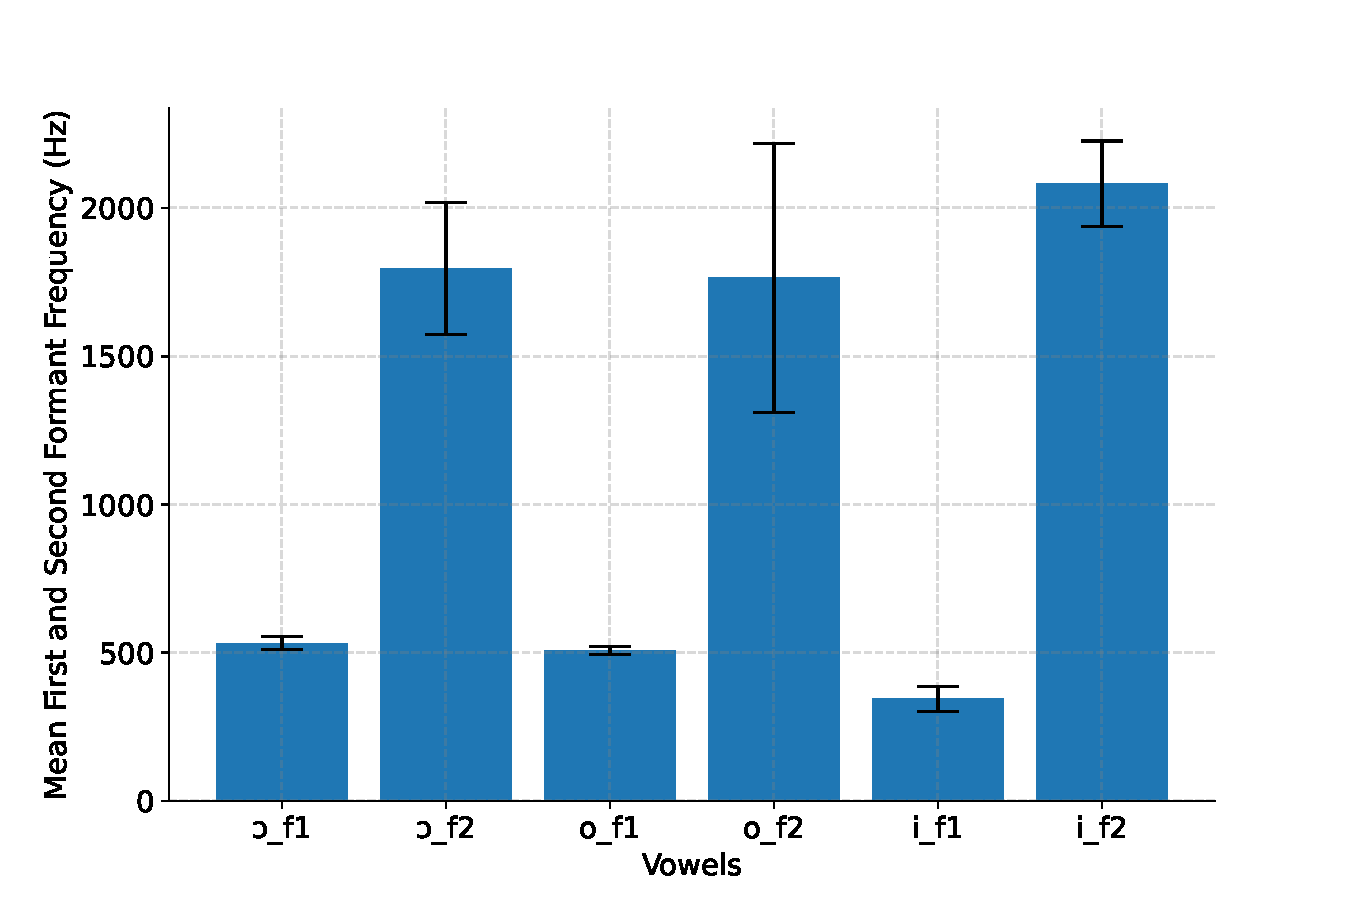
\includegraphics[width=9cm,height=5cm]{figures/IS2024_podobi_train_errorbar.pdf}};

\node[inner sep=0pt,anchor=center] (main_fig) at (10,20) % {x,y} from left corner in an imagined grid
{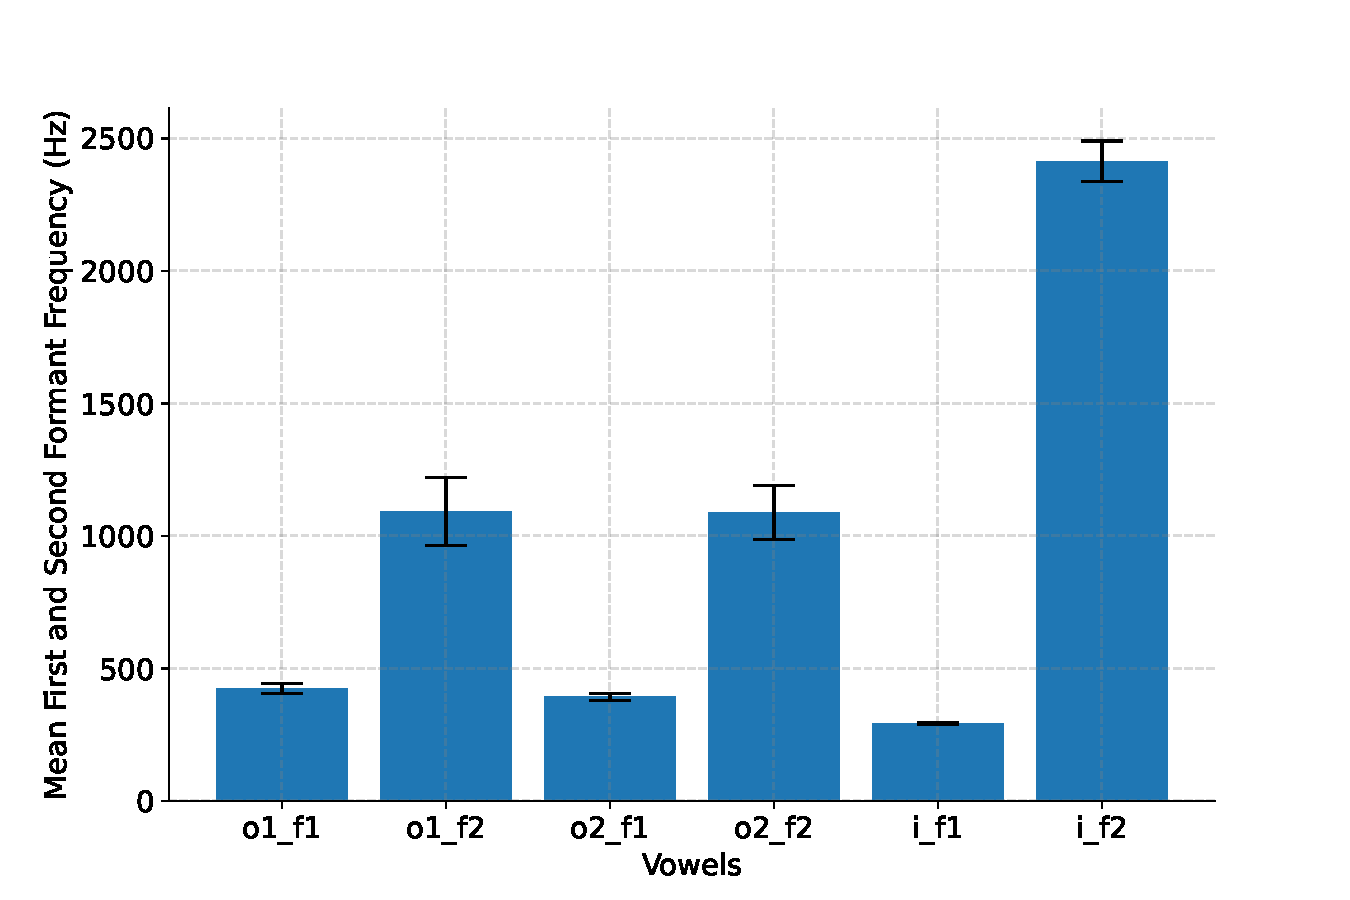
\includegraphics[width=9cm,height=5cm]{figures/IS2024_podobi_machine_errorbar.pdf}};


% ----- put axis labels
\node[font=\fontsize{8}{6}\selectfont,rotate=0,anchor=center] at (2,17.5) (l1) {(a)};
\node[font=\fontsize{8}{6}\selectfont,rotate=0,anchor=center] at (10,17.5) (l1) {(b)};

\end{tikzpicture}
